% Document settings

% Common
\DocumentMetadata{pdfversion=1.7, pdfstandard=A-2u}
\documentclass[11pt,letterpaper]{article}
\usepackage{fancyhdr}
\usepackage[]{fncychap}
\usepackage{etoolbox} % patch stuff
\usepackage[margin=1in]{geometry}
\usepackage{multirow}
\usepackage{longtable,booktabs} % typesetting
\usepackage{bookmark}
\usepackage[acronym]{glossaries-extra}
\pagestyle{plain}
\usepackage{parskip, setspace}

% Plots and Color
\usepackage{graphicx}
\usepackage{xcolor,colorspace}
\usepackage{tcolorbox}
\usepackage{pgfplots}
\pgfplotsset{compat=1.18} % Latest
\usepackage{epstopdf}
\usepackage[american voltages]{circuitikz}
\graphicspath{{images/}{drawings/}}

% Math stuff
\usepackage{mathtools} % loads amsmath and fixes its bugs, empheq, etc
\usepackage{amssymb}
\usepackage{sympytex}
\usepackage{siunitx}
\sisetup{detect-all=true}   % ensure proper font weight
\sisetup{per-mode = repeated-symbol}    % ensure "/" unit delineator
\sisetup{range-phrase = --,range-units = brackets} % hyphenated ranges, SI syntax
\DeclareMathSymbol{\varOmega}{\mathalpha}{operators}{"0A}   % upright omega for ohms
\providecommand*{\Ohm}{\varOmega}   % for siunitx
\DeclareSIUnit\sq{\ensuremath{\Box}}    % sheet resistance
\DeclareSIUnit{\Siemens}{S}
\DeclareSIUnit{\torr}{Torr} % add torr to siunitix 3
\DeclareSIUnit\sig{\ensuremath{\sigma}}

% Font
\usepackage{fontspec}
\setmainfont{STIXTwoText}[
	Extension		= .otf,
	UprightFont		= *-Medium,
	BoldFont		= *-Bold.otf,
	ItalicFont		= *-MediumItalic.otf,
	BoldItalicFont 	= *-BoldItalic.otf
]
\usepackage[math-style=ISO]{unicode-math}
\setmathfont{STIXTwoMath-Regular.otf} % for symbols
\usepackage{microtype}
\UseMicrotypeSet[protrusion]{basicmath} % disable protrusion for tt fonts
\urlstyle{same}

\usepackage[normalem]{ulem} % Enable normal \ul underline
\usepackage{fancyvrb}

\RequirePackage[type={CC},modifier={by-nc-nd},version={4.0},lang={english}]{doclicense}

\usepackage{datetime2} % to satisfy the "\today" in \hypersetup
\DTMusemodule{english}{en-US}
\usepackage{hyperref}
\hypersetup{
    hyperindex=true,
    colorlinks=true,
	bookmarksnumbered,
    bookmarksopen=true,
    linkcolor=blue,
    filecolor=magenta,      
    urlcolor=cyan,
%%%%%%%%%%%%%%%% METADATA %%%%%%%%%%%%%%%%%%%%	
    pdftitle={EE726 Project 2},
	pdfsubject={RTR StrongARM Comparator},
    pdfauthor={Chris Biancone},
	pdfpublisher={Chris Biancone},
	pdfkeywords={rail-to-rail, StrongARM, comparator, dynamic},
%%%%%%%%%%%%%%%%%%%%%%%%%%%%%%%%%%%%%%%%%%%%%%
	pdfproducer=pdfTeX-1.40.25,
	pdfdate=\today,
	pdflang={en},pdfmetalang={en},
	pdflicenseurl={},
    pdfpagemode=FullScreen,
}
\usepackage[nameinlink,capitalize]{cleveref}
\newcommand*{\doi}{}
\makeatletter
\newcommand{\doi@}[1]{\href{https://doi.org/#1}{#1}}
\DeclareRobustCommand{\doi}{\hyper@normalise\doi@}
\makeatother

% % % % % % % % % % % Header footer
% % % % % % % % % % %EDIT THIS % % % % % % % % % % % % % % % % % % % %
\pagestyle{fancy}
\fancyhf{}
\lhead{Tech Memo:  Project 2}
\rhead{Chris Biancone}
\lfoot{EE726}
\cfoot{\today }
\rfoot{Page \thepage}
% % % % % % % % % % % % % % % % % % % % % % % % % % % % % % % % % % % % %

% Scale images if necessary, so that they will not overflow the page
% margins by default, and it is still possible to overwrite the defaults
% using explicit options in \includegraphics[width, height, ...]{}
%\setkeys{Gin}{width=\maxwidth,height=\maxheight,keepaspectratio}

% No paragraph indent
\setlength\parindent{0pt}

\begin{document}

\VerbatimFootnotes % allows verbatim text in footnotes

\numberwithin{equation}{subsection}
\numberwithin{figure}{subsection}

	\hspace{5in}
	\includegraphics[scale=0.9,trim=0cm 0in 0in 0.0in,clip]{images/RIT_KGCOE1}
\newline

\Huge\textbf{EEEE 726: Project 2 \\RTR StrongARM Comparator}\\

\Large
\textbf{From:} Chris Biancone \\
\textbf{To: } Dr. Mark Pude \\
\textbf{Date: } 02/27/2024 \\
\textbf{Subject: } Project 2\\
\vspace{0.5in}

\section*{Abstract}
\normalsize
The purpose of this project is to design a comparator to given specifications for subsequent use in flash and SAR ADC projects. A comparator based on the established StrongARM topology and modified for rail-to-rail operation has been constructed in the Cadence gpdk045\_v5.0 PDK using \qty{2}{\V} CMOS devices. The comparator is followed by an SR latch to produce a valid output for the entire clock cycle, with appropriate buffering to drive a \qty{1}{\pF} load. The presented design achieves a nominal \qty{16.44}{\mV} hysteresis with \qty{1.22}{\mV} resolution and \qty{1.426}{\ns} propagation delay when sampling at the given target of \qty{12}{\MHz} for schematic level simulations. These results are achieved at a quiescent current draw of \qty{258}{\pA} for the entire design after stabilizing, with \qty{29.3}{\pA} contributed by the comparator itself. The design consumes an approximate \qty{1.06}{\pico\W} per decision. The performance is verified with minimal degradation in performance post-RC extraction across 60 PVT corners with 95\% yield in monte carlo mismatch simulation.

\section{Design Methodology}

\subsection{Circuit Topology}

The StrongARM dynamic comparator is a popular power-saving comparator circuit design, known to be suitable for all seasons. By incorporating a clock at this stage in the signal chain, either all NMOS or PMOS sources are turned off for half of the input clock cycle, thereby minimizing quiescent power draw. Its comparison performance relies almost entirely on careful design of its constituent devices' parasitic capacitances~\cite{Razavi2015}. During the reset phase of operation, all 4 internal nodes (\(X_1\), \(X_2\), \(O_1\), and \(O_2\)) are charged up to \(VDD\). At the beginning of the decision phase on the rising clock edge, the input pairs begin to turn on, a differential in voltage \(\Delta V_X\) is produced relative to the voltage differential at the inputs and the resulting discharge path resistance at (\(X_1\) and \(X_2\). The relationship of this change to the input device parameters is shown in \cref{eq:1}, omitting an additional term for non-ideal reset voltage (<\(VDD\)).

\begin{equation}
    \Delta V_{X(ideal)} = \frac{-g_m r_o + sC_{gd}r_o}{1+s\tau_a}\Delta V_{in},\; \tau_a = r_o(C_{gd}+C_{gs})
    \label{eq:1}
\end{equation}

As the nodes continue to drop, the cross-coupled (XCP) NMOS pair turns on and produces a \(\Delta V_O\). These nodes begin to fall as well with \(\Delta V_O\) rapidly increasing, finally turning on the PMOS cross-coupled pair. The positive feedback from the XCPs takes hold of the voltage difference and snaps the output nodes \(O_1\) and \(O_2\) to the appropriate voltage rail. The reset/regen phase then serves to charge up the parasitic capacitances back to \(VDD\), ready to make the next decision.

 \begin{figure}[htbp!]
		\centering
		\includegraphics[width=4in]{images/rtrcomp.png}
		\caption{StrongARM comparator with additional devices to achieve rail-to-rail operation, reproduced from~\cite{Qadasi2020}.}
		\label{Fig:rtrcomp}
	\end{figure}

The design presented here is based largely on the recent work of M. A. Al-Qadasi et.\ al~\cite{Qadasi2020}, which adds a complementary PMOS input pair to handle signals with a common mode voltage below the processing capability of the NMOS input pair, as shown in \cref{Fig:rtrcomp}. Additionally, two NMOS devices are added in parallel with the input and attached to the cross-coupled devices, such that as \(\Delta V_X\) grows, the NMOS device acts as a shunt to shut off the discharge path through the PMOS device that is on and prevent undetermined behavior. The NMOS devices are ideally of a lower threshold, to avoid operation specifically when only the PMOS devices are processing an input, but no 2V-LVT devices are available in the gpdk045.

Since this comparator makes a decision on each rising clock edge and resets on the falling edge, its output is invalid for half of the clock period. To remedy this, the output is fed to a standard SR latch with a logic buffer in between for decoupling the sensitive parasitic capacitances of the comparator. The output of this then mimics the behavior of a standard continuous-time design from the viewpoint of a receiving circuit.

\subsection{Calculations}

This design's reliance on the charging and discharging of parasitic capacitances, instead of the current steering of a standard comparator, provides atypical complexities when designing to specifications laid out for a continuous-time comparator. Notably, there is no DC operation of the dynamic comparator, so any DC characteristics like hysteresis must be estimated from a transient simulation. Meanwhile, standard device sizing methodologies like \(g_m/I_D\) do not apply as heavily as the design moves toward the digital realm. Few published works detail a concrete calculation of hysteresis voltage for a dynamic comparator, likely due to a pseudo-hysteresis implemented simply through the use of a clock to take discrete samples; Leïla Khanfir's recent publications surrounding her work on dynamic comparators with adjustable hysteresis provided a large basis of understanding for creating this design~\cite{Khanfir2018,Khanfir2019,Khanfir2020_1,Khanfir2021}. 

For a linearly varying input, it can be shown that the hysteresis of the comparator is dependent on no less than 4 variables: \(T_{reset}\) (clock low), input voltage slope \(a\), \(V_{cm}\), and transistor parameters:

\begin{equation}
    V_{HY}\bigg\rvert_{\Delta v_{in}(t) = at} = 2\left[\dfrac{C_{IX} + C_{XB}}{C_{int}}\Delta V_{tc0,X} exp\left(\dfrac{-t_{c1}}{\tau_{a}}\right) + \dfrac{C_{OB}}{C_{int}}\Delta V_{tc0,O} \right] + 2a\dfrac{g_m \tau_a \tau_b}{C_int} \left(1 - exp\left(\dfrac{-t_{c1}}{\tau_a}\right)\right)
    \label{eq:2}
\end{equation}

where \(C_{int}\) is a function of internal capacitors and \(t_{c1}\) is the time at which the comparator starts operating. Substituting the defined function for \(C_{int}\) allows finding \(V_{HY}\) as a function of these internal capacitances, which shows a greater sensitivity to the capacitances introduced at (\(X_1\), \(X_2\) (and their charging rates). This becomes useful when determining where to increase device sizes to increase yield over monte carlo simulations.


With a \qty{12}{\MHz} clock as a reference point, minimum device sizes are selected wherever possible, to allow for the fastest device operation and the ability to apply the final design to faster ADC circuits. While the StrongARM architecture has been proven in the gpdk045, this was done with \qty{1}{\V} devices that feature a minimum length of \qty{45}{\nm}~\cite{Dutta}. The minimum length of \qty{150}{\nm} for 2V devices is already sizeable at \qty{150}{\nm}, and will contribute to slowing down the discharge of the capacitors due to the increased resistance seen at each node of the circuit. For matching, the input NMOS are selected to have 4 \qty{320}{\nm} fingers of minimum size, so that the input PMOS devices and corresponding NMOS shunt devices may be half their size to avoid undetermined behavior. The tail switch and NMOS XCP devices are chosen to have 6 fingers, for resistance matching to the equivalent input stage. All of the PMOS sources are chosen to be minimum size with 2 fingers.


For the inverters and SR latch, all devices were initially conceived with 2 fingers at minimum size, which continued to work throughout simulation analysis. Shown in \cref{fig:comp-sch}, the lengths of the input devices were increased to \qty{1}{\um} following monte carlo simulations and a sensitivity analysis, to increase yield. The full schematic is shown in \cref{fig:full-sch}.

\begin{figure}[htbp]
    \centering
    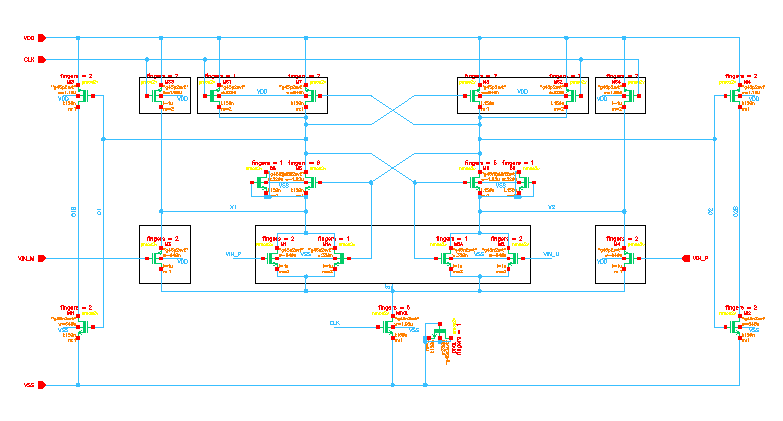
\includegraphics[width=\textwidth]{images/sch_comp.eps}
    \caption{Schematic of RTR StrongARM comparator.}
    \label{fig:comp-sch}
\end{figure}

\begin{figure}[htbp]
    \centering
    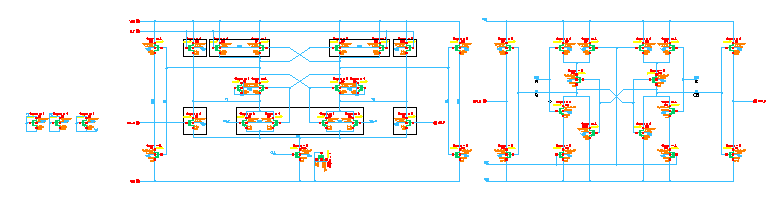
\includegraphics[width=\textwidth]{images/sch_full.eps}
    \caption{Schematic showing the comparator, inverters, and SR latch. Dummy devices used for layout are shown.}
    \label{fig:full-sch}
\end{figure}

\section{Schematic Level Simulations}

Schematic simulations were performed over PVT corners and monte carlo analysis. The process corners used were tt, ss, sf, fs, and ff, temperatures of 0, 27, 40, and \qty{85}{\degree\C}, and supply voltages of 1.8, 2.0, and \qty{2.2}{\V}. The schematic was captured and simulated using C\=adence Virtuoso.

\subsection{Hysteresis Testbench}

As mentioned, all aspects of this comparator must be analyzed using a transient simulation due to its clocked operation. Testbenches were set up using the same schematic shown in \cref{fig:tb-sch}, but varying the input \emph{vsource} and clock period. The clock was simulated using an ideal pulse with 5\% rise and fall time. Based on the work done in \cite{Khanfir2020_1}, a differential linear ramp was selected at a slope of \qty{200}{\mV\per\us} to function as a slowly-varying input compared to the \qty{12}{\MHz} clock source. 

\begin{figure}[!t]
    \centering
    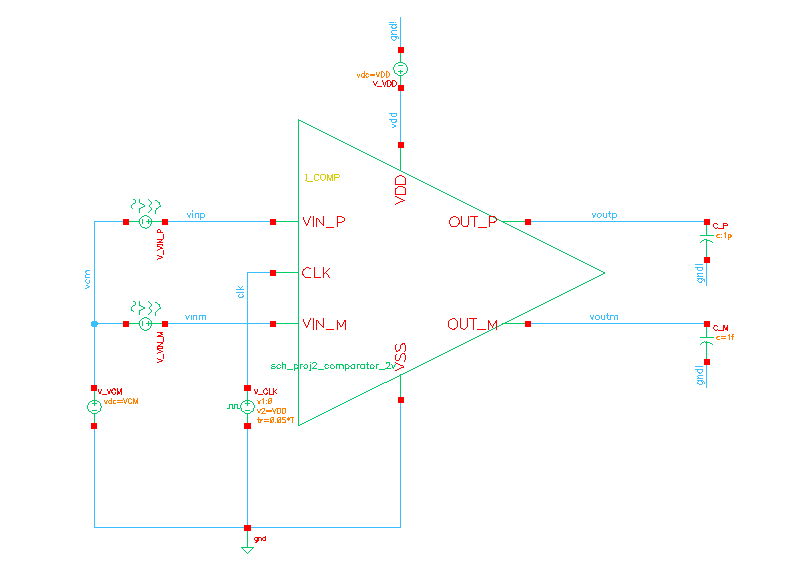
\includegraphics[width=4in]{images/sch_tb_prop_hyst.eps}
    \caption{Testbench setup used for all analyses.}
    \label{fig:tb-sch}
\end{figure}

The voltage at the positive input of the comparator was measured when the positive output both rose and fell, and the difference in the input voltage was determined to be the hysteresis.

\begin{figure}[!t]
    \centering
    \includegraphics[width=\textwidth]{images/hyst_plot.png}
    \caption{Hysteresis waveform.}
    \label{fig:hyst-plot}
\end{figure}

\subsection{Propagation Delay and ICMR Testbench}

To analyze propagation delay, the piece-wise linear inputs were changed to pulse inputs of \qty{12.5}{\mV} magnitude, resulting in a total differential of \qty{25}{\mV}. The inputs were arranged such that the crossover occurred just before the clock rising edge. Since the testbench was set up with a DC common mode voltage source, this was varied using parametric simulation to determine that the rail-to-rail operation was achieved and estimate the range. An example waveform is shown in \cref{fig:prop-plot}.

\begin{figure}[htbp!]
    \centering
    \includegraphics[width=\textwidth]{images/prop_icmr.png}
    \caption{Propagation delay test output, showing varied input common mode voltage.}
    \label{fig:prop-plot}
\end{figure}

As mentioned previously, the hysteresis of the dynamic comparator is known to be dependent on the reset time given to it. Often, this is achieved by simply running the comparator near its maximum speed, but to avoid the extra power consumption required to do this, using a PWM clock to dynamically change the hysteresis was explored in simulations. The ability to achieve a nearly \qty{120}{\mV} range of hysteresis was found; however, this required tight control of the clock pulse width near 90\% duty cycle. This was an interesting finding, but beyond the scope of this project for now. This principle is somewhat supported by \cite{Khanfir2018,Khanfir2021}, where a 4-bit clock delay is implemented for the output buffers of the comparator to form a pseudo-schmitt trigger, but further investigation is needed on the viability of PWM clocking.  

\subsection{Resolution}

Resolution was determined alongside the maximum reliable operation frequency the comparator could operate at. This was achieved simply by reducing the period of the clock within the hysteresis testbench setup.

\subsection{Results}

After sizing the devices and performing initial simulations, a sensitivity analysis for random mismatch was run to determine the biggest contribution to poor monte carlo results. \cref{fig:sense-results} shows that the circuit was most sensitive to variations in the input devices and PMOS switches MS3 and 4, which aligns with the expectation in \cref{eq:2} as these contribute to the capacitance and resistance at \(X_1\) and \(X_2\). Increasing the lengths of these devices to \qty{1}{\um} greatly increased the yield, and simulations were continued with these new values.

The comparator was able to easily achieve all design specification across corners at the schematic level. The schematic PVT corner results are summarized in \cref{tab:sch_corners}.

\begin{table}[]
    \centering
    \begin{tabular}{c|c|c|c|c|c}
    \toprule
        Parameter & Units & Spec & Nominal & Min & Max \\
    \midrule
        Hysteresis & mV & 10-20 & 16.4434 & 16.31 & 16.7834 \\
        Prop. Delay (\qty{1}{\pF}) & ns & 10 & 1.5184 & 1.1999 & 2.3522 \\
        Prop. Delay (\qty{1}{\fF}) & ps & - & 395.17 & 203.73 & 645.72 \\
        Resolution & mV & <25 & 1.21953 & 0.546049 & 3.49453 \\
        DC Current & nA & minimize & 0.25816 & 0.087434 & 9.0544 \\
        W/decision & pW & - & 1.0667 & 0.4653 & 2.3157 \\
        ICMR & mV & - & - & -200 & 2200 \\
        Layout Area & \(\qty{}{\um^2}\) & - & 180 & - & - \\
    \bottomrule
        
    \end{tabular}
    \caption{PVT corner results.}
    \label{tab:sch_corners}
\end{table}

The monte carlo mismatch analysis resulted in an overall yield of 98\%, with details shown in \cref{tab:sch_mc}.

\begin{table}[]
    \centering
    \begin{tabular}{c|c|c|c|c|c}
    \toprule
        Parameter & Units & Mean & Min & Max & Std Dev \\
    \midrule
        Hysteresis & mV & 16.6463 & 16.4731 & 33.0679 & 1.65875 \\
        Prop. Delay (\qty{1}{\pF}) & ns & 1.6106 & 1.5978 & 1.6346 & 0.0055696 \\
    \bottomrule
        
    \end{tabular}
    \caption{Monte carlo results.}
    \label{tab:sch_mc}
\end{table}

\begin{figure}[t!]
    \centering
    \includegraphics[width=\textwidth]{images/tp_avg_1p_mc.png}
    \caption{Propagation delay monte carlo histogram.}
    \label{fig:mc-plot}
\end{figure}

\begin{figure}[t!]
    \centering
    \includegraphics[width=\textwidth]{images/mc sensitivity analysis 1.png}
    \caption{Sensitivity analysis to monte carlo mismatch.}
    \label{fig:sense-results}
\end{figure}

\section{Layout}

Layout of the comparator was successfully accomplished with clean LVS and DRC - no errors in either. Much struggle was had while using the gpdk pcells, they resulted in many off-grid errors seemingly caused by themselves moving by \qty{1}{\nm} in random directions, which then pushed routes off by the same amount. Additionally, the dummy devices for the PMOS input pair were generated without contact cuts, and when abutted with the active devices, actually removed the contacts from the active devices. This was not caught for a while due to initially having M1-M2 contacts covering these areas. The final layout is shown in \cref{fig:layout}. The design is \qty{16.1}{\um} by \qty{9.96}{\um}.

\begin{figure}[!t]
    \centering
    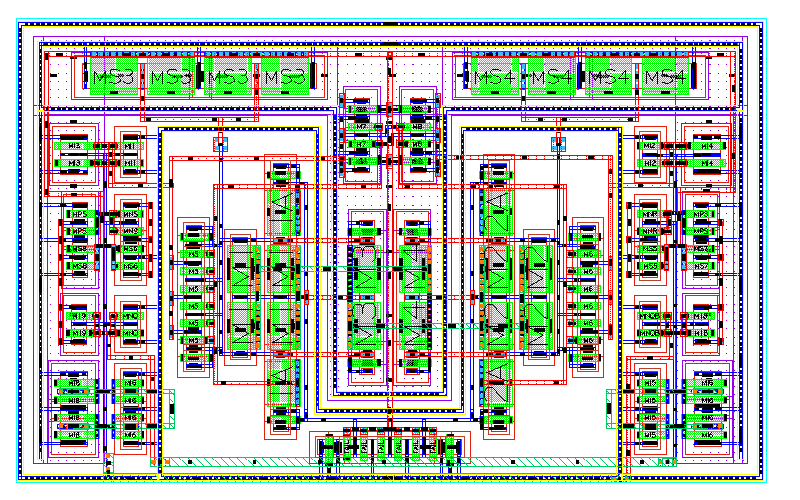
\includegraphics[width=\textwidth]{images/layout.eps}
    \caption{Comparator layout. The modified StrongArm buffer is centered, while the SR latch and buffer transistors are placed along the left and right sides.}
    \label{fig:layout}
\end{figure}

A solid guard ring is placed around the comparator PMOS and NMOS devices to shield these devices from noise, which did substantially complicate the routing. Metal 3 was used sparingly for the inputs and to bridge two nodes shared within the SR latch.

\section{Extracted Results}

Layout parasitic extraction was performed using Quantus PVS, using the typical RCx setting with decoupled capacitance referenced to \(VSS\). The resolution testbench could not be simulated across corners due to the amount of time it was taking; however, the hysteresis and propagation delay tests were simulated with close agreement to the schematic level simulations, verifying the robustness of the layout. These results are summarized in \cref{tab:ext_corners}.

\begin{table}[!t]
    \centering
    \begin{tabular}{c|c|c|c|c|c}
    \toprule
        Parameter & Units & Spec & Nominal & Min & Max \\
    \midrule
        Hysteresis & mV & 10-20 & 16.5203 & 16.3701 & 16.9196 \\
        Prop. Delay (\qty{1}{\pF}) & ns & 10 & 1.709 & 1.3403 & 2.6746 \\
        Prop. Delay (\qty{1}{\fF}) & ps & - & 558.45 & 344.51 & 915.93 \\
        DC Current & nA & minimize & 0.36671 & 0.20815 & 9.5295 \\
        W/decision & pW & - & 1.1326 & 0.5327 & 2.3975 \\
        ICMR & mV & - & - & -200 & 2200 \\
        Layout Area & \(\qty{}{\um^2}\) & - & 160 & - & - \\
    \bottomrule
        
    \end{tabular}
    \caption{Extracted corner results.}
    \label{tab:ext_corners}
\end{table}

Post-layout monte carlo simulation showed a 95\% yield for \qty{3}{\sig} variation, which was quite acceptable for this project's requirements. Results are summarized in \cref{tab:ext_mc}.

\begin{table}[!t]
    \centering
    \begin{tabular}{c|c|c|c|c|c}
    \toprule
        Parameter & Units & Mean & Min & Max & Std Dev \\
    \midrule
        Hysteresis & mV & 17.04 & 16.5334 & 33.1274 & 2.84316 \\
        Prop. Delay (\qty{1}{\pF}) & ns & 1.7592 & 1.7443 & 1.8072 & 0.010835 \\
    \bottomrule
        
    \end{tabular}
    \caption{Extracted monte carlo results.}
    \label{tab:ext_mc}
\end{table}

Waveforms for extracted simulations are shown in \cref{fig:ext_hyst_wav,fig:ext_prop_wav,fig:ext_current_wav}.

\begin{figure}[!t]
    \centering
    \includegraphics[width=\textwidth]{images/ext_hyst.png}
    \caption{Extracted hysteresis waveform.}
    \label{fig:ext_hyst_wav}
\end{figure}

\begin{figure}[!t]
    \centering
    \includegraphics[width=\textwidth]{images/ext_prop_icmr.png}
    \caption{Extracted propagation delay waveform.}
    \label{fig:ext_prop_wav}
\end{figure}

\begin{figure}[!t]
    \centering
    \includegraphics[width=\textwidth]{images/ext_current.png}
    \caption{Extracted transient current draw waveform.}
    \label{fig:ext_current_wav}
\end{figure}

\section{Conclusion}

This comparator design met all design specifications across corners post-layout, exceeding initial expectations. Adding the additional capability to process signals up to and exceeding the supply rails does not seem to be a thoroughly researched area for dynamic comparators, but the results from this experiment are very promising. This will prove to be a fortuitous addition for subsequent lab exercises, where this comparator will be implemented in a flash ADC requiring processing at $\frac{VDD}{2^4}$ increments. This comparator can be employed for each voltage level instead of using separate NMOS and PMOS input architectures, which should ensure better performance across the voltage range and from ADC to ADC.

\newpage

\bibliographystyle{bib/IEEEtranDOI}
\bibliography{bib/main.bib}

\end{document}